%%%%%%%%%%%%%%%%%%%%%%%%%%%%%%%%%%%%%%%
%----------------------------------------     网络中的增量图表征算法     ---------------------------------------%
%%%%%%%%%%%%%%%%%%%%%%%%%%%%%%%%%%%%%%%
\chapter{网络中的增量图表征算法}
\section{引言}
	社交网络的蓬勃发展使得信息网络研究领域面临越来越多的机遇和挑战。传统的网络特征的表示方法都是以邻接矩阵,拉普拉斯矩阵等离散型或者以中心度,出入度等人工规则来表达,然而在社交网络中随着网络节点的增加,这些表达方法的复杂度和有效性都会出现比较大的问题。近年来机器学习、人工智能的飞速发展,复杂信息网络也因此受益,对网络的表征学习吸引了越来越多的研究兴趣。类似于自然语言中的词向量表征的发展,单词的词频或逆文档频率(TF-IDF)等人工规则表征对于一个单词的描述太过简略,词向量表征则将单词映射成一个向量,向量之间可以计算相似度、并进行加减等操作,对于词的描述在数学意义上更加丰富,图表征学习也是需要从对网络的离散型或人工规则型表达发展出连续性且具有更丰富表征意义的向量表示算法。对于图表征得到的节点表征向量矩阵,需要应用于后续的机器学习任务,不同的机器学习任务对应不同的图挖掘问题,比如对节点向量进行聚类学习,相当于图挖掘领域的社区发现过程;对网络中连边进行分类任务,相当于图挖掘领域的链路预测任务。另外,图表征向量矩阵可用于计算相似度、节点分类、可视化、节点推荐等任务。
	
	本章将提出一种基于高阶接近度的图表征算法,并通过分析不同增量场景的模型变化,提出在增量场景下对应的表征算法。
	
\section{问题描述}
假设一个无向网络$G=(E,V)$,其中$V$表示网络$G$中节点的集合,$E$表示网络$G$中连边的集合,通常图是用邻接矩阵$A \in R^{|V|\times|V|}$表示的,图表征算法的定义就是通过寻找一个映射函数来表征网络中的每个节点:
\begin{equation}
f_G: \textbf{A} \rightarrow \textbf{X} \in R^{|V| \times k} \qquad s.t.\quad k<<|V|
\end{equation}
对于真实应用中的网络往往是存在动态变化的,对于传统的图表征算法来说,真实场景下的动态网络会带来很大的挑战,传统算法基本都是离线模型,当新数据进入时,需要重新对全部数据进行批量处理。在网络规模很大时,离线模型是不具备伸缩性的,也不适合于在线应用中使用。因此对于大型动态网络需要提出一种增量式的学习框架来实现快速、可扩展的表征学习。

为了方便描述统一字符使用规范及意义,用大写字母加粗表示矩阵,如$\textbf{A}$;用小写字母加粗表示向量,如$\textbf{a}$;用普通小写字母代表标量,如$a$;矩阵$\textbf{A}$的第$i$行用$\text{A}(i,:)$表示;矩阵$\textbf{A}$的第$j$列用$\textbf{A}(:,j)$表示,也可以简写为$\textbf{A}_j$;矩阵$\textbf{A}$中第$i$行第$j$列元素用$\textbf{A}(i,j)$表示,也可以简写为$\textbf{A}_{ij}$,矩阵$\textbf{A}$的转置记为$\textbf{A}^T$,矩阵$\textbf{A}$的迹记为$tr(\textbf{A})$,$\textbf{I}$代表单位矩阵;常用的字符表如下表:
\begin{table}
	\centering
	\caption{常用字符及其代表含义}
	\begin{tabular}{|C{1.8in}|C{3.3in}|}
		\hline
		\textbf{字符} & \textbf{含义} \\ \hline\hline
		$G^{(t)}$ & 时刻$t$时的网络数据 \\ \hline
		$G^{(t+1)}$& 时刻$t+1$时的网络数据  \\ \hline
		$\textbf{A}^{(t)}$ & 时刻$t$时网络的邻接矩阵 \\ \hline
		$\textbf{A}^{(t+1)}$ & 时刻$t+1$时网络的邻接矩阵 \\ \hline
		$\Delta\textbf{A}$ & 时刻$t$到时刻$t+1$之间邻接矩阵的变化 \\ \hline
		$\textbf{X}^{(t)}$ & 时刻$t$时网络的表征向量矩阵 \\ \hline
		% $\textbf{X}^{t+1}$ & 时刻$t+1$时网络的表征向量矩阵 \\ \hline
		$k$ & 节点向量表征的维数  \\ \hline
	\end{tabular}
\end{table}

用$V^{(t)} = \{v_1, v_2,\cdots,v_n\}$表示在时刻$t$网络$G^{(t)}$中的节点集合,用$\textbf{A}^{(t)}$来表示时刻$t$的网络结构,随着时刻$t$的变化,网络的拓扑结构会发生变化,当网络中节点数目不变时,用$\Delta\textbf{A}$表示邻接矩阵从时刻$t$到时刻$t+1$的变化;当网络中有新增节点的时候,需要对邻接矩阵$\textbf{A}^{(t)}$进行增广再计算变化量。如前文中提到的,在动态网络中重复用离线模型是不适合在线应用的,那么对于动态网络的学习过程应该分成两个部分:1.静态网网络的学习过程;2.增量网络的学习过程;也即转化成如下两个问题:
\begin{itemize}
	\item \textbf{问题1}:静态场景下的图表征算法。给定网络的邻接矩阵$\textbf{A}^{(t)}$,对于所有节点学习网络的表征向量矩阵$\textbf{X}^{(t)}$。
	\item \textbf{问题2}: 增量场景下的图表征算法。给定网络某时刻$t+1$的邻接矩阵$\textbf{A}^{(t+1)}$,
		和上一时刻的表征向量$\textbf{X}^{(t)}$,对于所有节点学习网络的表征向量矩阵$\textbf{X}^{(t+1)}$
\end{itemize}

下面章节将就这两个问题展开讨论分析。

%%%%%%%%%%%%%%%%%%%%%%%%%%%%%%%%%%%%%%%
%----------------------------------------     静态场景下的图表征算法     ---------------------------------------%
%%%%%%%%%%%%%%%%%%%%%%%%%%%%%%%%%%%%%%%

\section{静态场景下的图表征算法}
在图表征学习中,最早的方法借鉴与流形学习(manifold learning)的算法,其中Belkin和Niyogi提出的拉普拉斯特征映射是流形学习中的一种典型算法,该算法假设表征映射后得到的表征向量需要保证原网络中一阶接近度,也就是需要保证网络中互为邻居的节点对连边权重越大,那么在表征向量空间就应该保证越接近,也即优化如下问题:
\begin{equation}\label{laplacian_st}
\begin{aligned}
\min_{X^TDX=I} \phi(X) &= \frac{1}{2}\sum_{i,j}|X_i - X_j|^2A_{ij} \\
&= \frac{1}{2}(\sum_{i,j}(x_i^2+x_j^2-2x_ix_j) A_{ij}) \\
&=\frac{1}{2} (\sum_ix_i^2D_{ii} +\sum_j x_j^2 D_{jj} - 2\sum_{i,j}x_i x_j A_{ij}) \\
&= tr(X^TLX)
\end{aligned}
\end{equation}
其中$X$为表征向量矩阵,$A$为图的邻接矩阵,$D$为对角元素为节点度的对角阵,$L$为拉普拉斯矩阵。对式(\ref{laplacian_st}),根据谱图理论\cite{chung1997spectral}可以通过拉普拉斯算子的最值特征向量来进行逼近,上述问题可以转化为(推导过程如式(\ref{laplacian_reduce})):
\begin{equation}
\max_{X^TX = I} tr(X^TWX)
\end{equation}
其中$W = D^{-\frac{1}{2}}AD^{-\frac{1}{2}} $。为得到图表征向量就转变成求$W$矩阵的前$k$大的特征值所对应的特征向量。

拉普拉斯特征映射假设中只考虑到保留一阶接近度,对于图表征来说,一阶接近度所表征的信息是远远不够的,因此需要引进更高阶的接近度来表征向量,比如LINE算法引入了二阶接近度;DeepWalk算法引进了$l$(游走半径)阶接近度,对比实验也验证了在保留高阶接近度的算法中后续的节点分类等机器学习任务效果更好。

\subsection{基于高阶接近度的拉普拉斯特征映射}
在这一部分,主要集中在无向图中的图表征过程,因此在保证得到节点的表征向量的同时,对称性也在考虑之列。基于对称性这个基本假设,提出基于拉普拉斯特征映射改进的目标函数,用来保留高阶接近度:
\begin{equation}\label{high_order_condition}
%\begin{aligned}
	\min_{X^TD'X=I} \phi(X) = \frac{1}{2}\sum_{i,j}|X_i - X_j|^2S_{ij} 
%	&= \frac{1}{2}(\sum_{i,j}(y_i^2+y_j^2-2y_iy_j) S_{ij}) \\
%	&=\frac{1}{2} (\sum_iy_i^2D'_{ii} +\sum_j y_j^2 D'_{jj} - 2\sum_{i,j}y_i y_j S_{ij}) \\
%	&= tr(X^T(D'-S)X)
%\end{aligned}
\end{equation}
其中约束条件中的$D'$为区别于$S$矩阵为邻接矩阵时对应的对角矩阵$D$,根据不同的$S$矩阵进调整。$S$矩阵是通过保留高阶接近度的计算方法得到的,比如共同邻居(Common Neighbors,CN)\cite{newman2001clustering}、Adamic-Adar系数(AA)\cite{adamic2003friends}、资源分配系数(Resource Allocation,RA)\cite{zhou2009predicting}、Jaccard系数、Katz系数、个性化Pagerank(Personalized Pagerank)\cite{wang2015link}等方式,后文将称$S$矩阵为\textbf{相似度矩阵$S$}。下面将重点介绍前三种计算方法。

\definition{\textbf{共同邻居}:}
共同邻居计算方法是目前用来衡量节点接近度中使用最广泛的之一,因为这种计算非常简单,节点对$i$,$j$之间的共同邻居值就是跟$i$,$j$都有直接连边的节点数,也即:
\begin{equation}
	CN(i,j) = |N(i) \cap N(j)|
\end{equation}
其中$N(i)$表示节点$i$的邻居节点集合,$|\cdot|$表示对集合计数。将共同邻居这个计算方法推广至矩阵形式,可以得到用来保留高阶接近度的相似度矩阵$S_{CN}$:
\begin{equation}
	S_{CN}(A) = A^2 - D
\end{equation}
其中$A$为无向网络的邻接矩阵, $\textbf{D}$为节点度的对角矩阵。
\definition{\textbf{Adamic-Adar系数}:}Adamic-Adar系数最先是由Adamic和Adar提出来用来计算两个网页之间的相似度的,后来被广泛应用与社交网络分析之中。Adamic-Adar系数的计算方法类似于共同邻居,不同的是对不同的共同邻居采用不同的权重,该系数假定度较高的节点在共同邻居中所占权重较低,权重值为对数节点度的倒数,也即:
\begin{equation}
	AA(i,j) = \sum_{u \in N(i)\cap N(j)} \frac{1}{\log(|N(u)|)}
\end{equation}
其中$|N(u)|$也称为节点$u$的度。同样地,将Adamic-Adar系数计算方法推广至矩阵形式,在不考虑对角线元素的情况下,可以得到对应用来保留高阶接近度的相似度矩阵$S_{AA}$:
\begin{equation}
	S_{AA}(A) = A \cdot M \cdot A
\end{equation}
其中$M$为对角矩阵,且有:
\begin{equation}
M_{ii} = 1/\log(\sum_j{A_{ij}})
\end{equation}

\definition{\textbf{资源分配系数}:}资源分配系数最早是基于物理过程中的资源分配得来的一个计算法方法,过程类似于Adamic-Adar系数的计算方法,同样是给度较高的节点惩罚权重,资源分配系数采取的权重是节点度的倒数,因此可以看出来资源分配系数对度高的节点惩罚相较之下比较重,度处在平均水平的节点两中计算方法的惩罚权重相当。资源分配系数的计算方法如下:
\begin{equation}
	RA(i,j) =  \sum_{u \in N(i)\cap N(j)} \frac{1}{|N(u)|}
\end{equation}
同样地,在不考虑对角线元素的情况下,可以将资源分配系数推广至矩阵形式,得到矩阵$S_{RA}$:
\begin{equation}
	S_{RA}(A) = A\cdot K \cdot A
\end{equation}
其中$K$为对角矩阵,且有:
\begin{equation}
	K_{ii} = 1/\sum_jA_{ij}
\end{equation} 

根据以上三种系数的介绍和定义\ref{first_order}和定义\ref{second_order}中介绍的接近度概念,在共同邻居的计算方法中引入了二阶接近度,也即二度邻居的信息,在Adamic-Adar系数和资源分配系数中,不仅计算了共同邻居,还对共同邻居的度(邻居总数)进行了计算和处理,也即处理了高于二阶接近度的高阶接近度信息。为方便后文进行推导,可以将三种相似度矩阵$\textbf{S}$计算方法表达成统一的形式:
\begin{equation}\label{unify}
	\textbf{S} = \textbf{A} \cdot \textbf{M} \cdot \textbf{A}
\end{equation}
对应的三种相似度矩阵$S$的表格如下:
\begin{table}
	\centering
	\caption{三种相似度矩阵计算方法}
	\begin{tabular}{|C{1.0in}|C{1.8in}|C{1.8in}|}
		\hline
		$\textbf{S}$ & 表达式 & $\textbf{M}$的值  \\ \hline\hline
		$\textbf{S}_{CN}$ & $\textbf{A}\cdot \textbf{M}_{CN} \cdot\textbf{A}$ & $\textbf{I}$  \\ \hline
		$\textbf{S}_{AA}$ & $\textbf{A}\cdot \textbf{M}_{AA}\cdot \textbf{A}$ & $\textbf{M}_{ii} = 1/\log(\sum_j{\textbf{A}_{ij}})$ \\ \hline
		$\textbf{S}_{RA}$ & $\textbf{A}\cdot \textbf{M}_{RA}\cdot \textbf{A}$ & $\textbf{M}_{ii} = 1/\sum_j\textbf{A}_{ij}$ \\ \hline
	\end{tabular}
\end{table}

考虑式\ref{high_order_condition},当采用不同的相似度矩阵$S$时,$D'$满足:
\begin{equation}
D'_{ii} = \sum_j{S_{ij}}
\end{equation}
于是同式(\ref{laplacian_reduce})推导,则原问题变成:
\begin{equation}\label{decomp}
\max_{X^TX = I} tr(X^TWX)
\end{equation}
其中$W = D^{\prime-\frac{1}{2}}SD^{\prime-\frac{1}{2}}$,上述问题转化为求矩阵$W$的特征值问题,也即对矩阵$W$进行特征值分解:
\begin{equation}\label{evol}
	W = X^T \Lambda X 
\end{equation}
其中$\Lambda$为对角矩阵,对角线元素为矩阵$W$的特征值,$X$为正交矩阵,也即表征向量矩阵。对于式(\ref{decomp})的最大值问题相当于求解$W$最接近特征值分解形式,也即矩阵$X$为$W$前$k$个特征值对应的特征向量组合而成的矩阵。

\subsection{HLE算法描述}
	给定图数据$G = (E,v)$和图表征向量维数$k$,其中图$G$以邻接矩阵$A\in R^{|V|\times |V|}$表示,HLE算法将得到图$G$的向量表征$X\in |V|\times k$。
	
	在算法开始时,根据相似度准则的选择,令相似度矩阵$S$分别为共同邻居$S_{Cn}$、Adamic-Adar系数$S_{AA}$或资源分配系数$S_{RA}$中的一个。根据$S$矩阵计算出对应的对角矩阵$D\prime$,使得$D'_{ii} = \sum_j S_{ij}$。

	进一步计算矩阵$W$,使得$W=D^{\prime-\frac{1}{2}}SD^{\prime-\frac{1}{2}}$,对W矩阵进行特征值分解得到前k个最大特征值对应的特征列向量$\{X_1,X_2,\cdots,X_k\}$,组合成图表征向量矩阵$X$。
	
	HLE算法中根据不同的接近度要求可以选择不同的相似度计算方法,其中共同邻居保留二阶接近度,Adamic-Adar系数和资源分配系数保留网络的三阶接近度。


%\algorithm{基于高阶接近度的拉普拉斯特征映射HLE}
\begin{figure}[htb]
	\centering
	\begin{minipage}{.7\linewidth}
		\begin{algorithm}[H]
			\small
			\caption{HLE算法}
			\begin{algorithmic}[1]
				\Require
				\Statex $\textbf{A}$ :邻接矩阵
				\Statex $k$ : 表征向量维数
				\Ensure
				\Statex $\textbf{X}$ :表征向量矩阵
				\Statex $\Lambda$:特征值对角矩阵
				\Statex
				\State $\mathcal{S} \leftarrow S_{CN}(A) /S_{AA}(A) / S_{RA}(A)$
				\State $D'_{ii} = \sum_j S_{ij}$
				\State $W \leftarrow  D^{\prime-\frac{1}{2}}SD^{\prime-\frac{1}{2}}$
				\State 通过特征值分解得到$W$前k个特征向量,组合成矩阵 $\textbf{X}$以及对应特征值组成的对角矩阵$\Lambda$
				\State 返回 $\textbf{X}$
			\end{algorithmic}
		\end{algorithm}
	\end{minipage}
\end{figure}
%%%%%%%%%%%%%%%%%%%%%%%%%%%%%%%%%%%%%%%
%----------------------------------------     增量场景下的图表征算法     ---------------------------------------%
%%%%%%%%%%%%%%%%%%%%%%%%%%%%%%%%%%%%%%%

\section{增量场景下的图表征算法}
前面一节提出了应用高阶接近度的拉普拉斯特征映射方法来对网络进行表征,对于真实应用中的网络往往是存在动态变化的。比如在社交媒体上,网络中时刻会存在用户进行更新状态、添加好友等操作,这些操作都是会引起社交关系发生变化的,从数学角度看就是网络中的连边会出现增删等情况;除此之外社交媒体中,也会存在有新的用户注册加入的情况,这种情况即对应网络中有新加入的节点。对于传统的图表征算法来说,真实场景下的动态网络会带来很大的挑战,传统算法基本都是离线模型,对于变化后的网络只能进行重新计算或学习,当网络规模很大时,离线模型是不具备伸缩性的,也不适合于在线应用中使用。因此对于大型动态网络需要提出一种增量式的学习方式来实现快速、可扩展的表征学习。

下面将提出一种增量的图表征算法,应用于增量场景下的图表征学习,在这里本文采用文献\cite{chi2007evolutionary}中采用的假设,认为在时刻$t$和时刻$t+1$之间网络的变化是平缓而微小的,可采用矩阵摄动理论\cite{stewart1990matrix}进行分析和处理。如前文中提到的,网络中的变化场景分两类:1. 节点数不变,网络连边的增删;2.节点新增;因此下面将分别就这两种情况进行分析和处理。
%%%%%%%%%%%%%%%%%%%%%%%%%%%%%%%%%%%%%%%
%----------------------------------------     节点数不变    ---------------------------------------%
%%%%%%%%%%%%%%%%%%%%%%%%%%%%%%%%%%%%%%%
\subsection{节点不变}
本文的研究对象是无向网络,根据式(\ref{evol}),在时刻$t$网络表征学习相当对矩阵$\textbf{W}^{(t)}$进行特征值分解,也即:
\begin{equation}
	\textbf{W}^{(t)} = \textbf{X}^{(t)T} \Lambda^{(t)} \textbf{X} ^{(t)}
\end{equation}
其中$\textbf{X} ^{(t)}$为时刻$t$是网络的表征向量,其中$\textbf{W}^{(t)} = \textbf{D}^{\prime(t)-\frac{1}{2}}\textbf{S}^{(t)}\textbf{D}^{\prime(t)-\frac{1}{2}}$;在网络节点不变的情况下,根据矩阵摄动理论\cite{stewart1990matrix},用$\Delta\textbf{W}$表示时刻$t$到时刻$t+1$网络变化引起的矩阵$\textbf{W}$的变化,则有
\begin{equation}
	\textbf{W}^{(t+1)} = \textbf{W}^{(t)} + \Delta\textbf{W}
\end{equation}
对矩阵$\Delta\textbf{W}$进行矩阵分解,则有:
\begin{equation}
	\Delta\textbf{W} =  \textbf{Y}^{T} \textbf{Z}  \textbf{Y}
\end{equation}
其中矩阵$\textbf{Z}$为对角矩阵,$\textbf{Y}$为$\Delta\textbf{W}$的特征向量矩阵,网络变化的定义,变化后的矩阵等于变化前的矩阵加上变量,即:
\begin{equation}\label{time_t1}
\begin{aligned}
\textbf{W}^{(t+1)} &= \textbf{X}^{(t+1)T} \Lambda^{(t+1)} \textbf{X} ^{(t+1)} \\
 &= \textbf{W}^{(t)} + \Delta \textbf{W} \\
&= \textbf{X}^{(t)T} \Lambda^{(t)} \textbf{X} ^{(t)} +  \textbf{Y}^{T} \textbf{Z}  \textbf{Y} \\
&= \begin{bmatrix} \textbf{X}^{(t)T} & \textbf{Y}^{T}\end{bmatrix}
   \begin{bmatrix}  \Lambda^{(t)} & \textbf{0}\\
   \textbf{0} & \textbf{Z}
   \end{bmatrix}
   \begin{bmatrix} \textbf{X}^{(t)} \\ \textbf{Y}\end{bmatrix} \\
&= \tilde{\textbf{X}}^{(t)T} 
\begin{bmatrix}  \Lambda^{(t)} & \textbf{0}\\
\textbf{0} & \textbf{Z}
\end{bmatrix}
\tilde{\textbf{X}}^{(t)}
\end{aligned}
\end{equation}
其中为方便表述,记$ \tilde{\textbf{X}}^{(t)T}= \begin{bmatrix} \textbf{X}^{(t)T} & \textbf{Y}^{T}\end{bmatrix}$。通过矩阵特征值分解的特性可知,矩阵$\textbf{X}^{(t)T}$为正交矩阵,那么对于时刻$t$所对应的表征向量矩阵$\textbf{X}^{(t+1)T}$也应是正交矩阵,为此需引入QR分解。
\definition{\textbf{QR分解}}:QR分解是线性代数中常用的矩阵分解方法,将矩阵$\textbf{A}$分解成两个矩阵的乘积,一个是正交矩阵$\text{Q}$,也即$\textbf{Q}^T\textbf{Q} = \textbf{I}$,一个是上三角矩阵$\textbf{R}$,也即当$i>j$时,有$\textbf{R}_{ij} =0$,当矩阵$\textbf{A}$为非奇异矩阵时,QR分解是唯一的,也即:
\begin{equation}
	\textbf{A} = \textbf{Q} \textbf{R}
\end{equation}
关于QR分解有很多计算方法,包括施密特(Gram-Schmidt)正交化过程,Householder变化,以及Givens旋转的方法。下面主要介绍通过施密特正交化过程进行QR分解。

\remark{施密特正交化过程}:
对于矩阵$\textbf{A}$做施密特正交化过程,其中矩阵$\textbf{A}$原始形式为:
\begin{equation}
	\textbf{A} = \begin{bmatrix} \textbf{A}_1 | & \textbf{A}_2 | & \cdots | & \textbf{A}_n \end{bmatrix}
\end{equation}

通过施密特正交化过程对原有矩阵$\textbf{A}$进行正交化,得到$\textbf{Q} = \begin{bmatrix} \textbf{Q}_1 | & \textbf{Q}_2 | & \cdots | & \textbf{Q}_n \end{bmatrix}$,其中$\textbf{Q}$为正交矩阵,则对应有:
\begin{equation}\label{Gram}
	\begin{aligned}
		\textbf{q}_1 &= \textbf{A}_1,\quad \textbf{Q}_1 = \frac{\textbf{q}_1}{|\textbf{q}_1|} \\
		\textbf{q}_2 &= \textbf{A}_2-(\textbf{A}_2\cdot\textbf{Q}_1)\textbf{Q}_1,\quad \textbf{Q}_2 = \frac{\textbf{q}_2}{|\textbf{q}_2|} \\
		\textbf{q}_n &= \textbf{A}_n-(\textbf{A}_{n}\cdot\textbf{Q}_1)\textbf{Q}_1-\cdots-(\textbf{A}_{n}\cdot\textbf{Q}_{n-1})\textbf{Q}_{n-1},  \quad\textbf{Q}_n = \frac{\textbf{q}_n}{|\textbf{q}_n|} \\
	\end{aligned}
\end{equation}
那么通过式(\ref{Gram}),可知QR分解可以通过施密特正交化进行迭代求解,于是进一步地可以推导出矩阵$\textbf{A}$和矩阵$\textbf{Q}$之间的关系如下:
\begin{equation}
\begin{aligned}
\textbf{A} &= \begin{bmatrix} \textbf{A}_1 | & \textbf{A}_2 | & \cdots | & \textbf{A}_n \end{bmatrix} \\
& = \begin{bmatrix} \textbf{Q}_1 | & \textbf{Q}_2 | & \cdots | & \textbf{Q}_n \end{bmatrix}
\begin{bmatrix}\textbf{A}_1\cdot\textbf{Q}_1 &  \textbf{A}_2\cdot\textbf{Q}_1 & \cdots & \textbf{A}_n\cdot\textbf{Q}_1 \\
0 & \textbf{A}_2\cdot\textbf{Q}_2 & \cdots & \textbf{A}_n\cdot\textbf{Q}_2 \\
\vdots & \vdots & \ddots & \vdots \\
0& 0 & \cdots &\textbf{A}_n\cdot\textbf{Q}_n
\end{bmatrix}  \\
&= \textbf{Q}\textbf{R}
\end{aligned}
\end{equation}


引入使用施密特正交化进行QR分解后,对式子(\ref{time_t1})中矩阵$\tilde{\textbf{X}}^{(t)T} = \begin{bmatrix} \textbf{X}^{(t)T} & \textbf{Y}^{T}\end{bmatrix}$进行QR分解。通过前置条件已知$\textbf{X}^{(t)T}$为正交矩阵,对$\tilde{\textbf{X}}^{(t)T}$的分解只需要对矩阵$\textbf{Y}^{T}$进行进一步施密特正交化完成QR分解,记$\textbf{X}^{(t)T}=\begin{bmatrix} \textbf{X}^{(t)T}_1 | & \textbf{X}^{(t)T}_2 | & \cdots | & \textbf{X}^{(t)T}_k \end{bmatrix}$,$\textbf{Y}^{T}=\begin{bmatrix} \textbf{Y}^T_1 | & \textbf{Y}^T_2 | & \cdots | & \textbf{Y}^T_m \end{bmatrix}$,则有:
\begin{equation}\label{delta}
\begin{aligned}
\tilde{\textbf{X}}^{(t)T} &= \begin{bmatrix} \textbf{X}^{(t)T} & \textbf{Y}^{T}\end{bmatrix} \\
&=\begin{bmatrix} \textbf{X}^{(t)T}_1 | & \textbf{X}^{(t)T}_2 | & \cdots | & \textbf{X}^{(t)T}_k| \textbf{Y}^T_1 | & \textbf{Y}^T_2 | & \cdots | & \textbf{Y}^T_m \end{bmatrix} \\
&= \begin{bmatrix} \textbf{X}^{(t)T}_1 | & \cdots | & \textbf{X}^{(t)T}_k| \textbf{X}^{(t)T}_{k+1} | &\cdots|& \textbf{X}^{(t)T}_{k+m} \end{bmatrix}
\begin{bmatrix}1 &  0 & \cdots & \textbf{Y}^T_1\cdot\textbf{X}^{(t)T}_{1} & \cdots & \textbf{Y}^T_m\cdot\textbf{X}^{(t)T}_{1}\\
0 & 1  & \cdots & \textbf{Y}^T_1\cdot\textbf{X}^{(t)T}_{2} & \cdots & \textbf{Y}^T_m\cdot\textbf{X}^{(t)T}_{2}\\
\vdots & \vdots & \ddots & \vdots  & \ddots & \vdots \\
0& 0 & \cdots & 0 & \cdots &  \textbf{Y}^T_m\cdot\textbf{X}^{(t)T}_{n}
\end{bmatrix}  \\
&= \begin{bmatrix} \textbf{X}^{(t)T} & \Delta\textbf{Q}^{T} \end{bmatrix}
 \begin{bmatrix} \textbf{I} & \textbf{R}_1 \\
 0 & \textbf{R}_2
 \end{bmatrix}
\end{aligned}
\end{equation}
其中$\textbf{X}^{(t)T}_{k+i}$可根据式(\ref{Gram})推导出,$\Delta\textbf{Q}^{T} =\begin{bmatrix}  \textbf{X}^{(t)T}_{k+1} | &\cdots|& \textbf{X}^{(t)T}_{k+m} \end{bmatrix}$

进一步地将式(\ref{delta})代入式(\ref{time_t1})中,则原问题转换成:
\begin{equation}\label{time_t2}
	\begin{aligned}
	\textbf{W}^{(t+1)} &= \textbf{X}^{(t+1)T} \Lambda^{(t+1)} \textbf{X} ^{(t+1)} \\
	&= \tilde{\textbf{X}}^{(t)T} 
	\begin{bmatrix}  \Lambda^{(t)} & \textbf{0}\\
	\textbf{0} & \textbf{Z}
	\end{bmatrix}
	\tilde{\textbf{X}}^{(t)} \\
	&= \begin{bmatrix} \textbf{X}^{(t)T} & \Delta\textbf{Q}^{T} \end{bmatrix}\begin{bmatrix} \textbf{I} & \textbf{R}_1 \\
	0 & \textbf{R}_2 \end{bmatrix}
	\begin{bmatrix}  \Lambda^{(t)} & \textbf{0}\\
	\textbf{0} & \textbf{Z} \end{bmatrix}
	\begin{bmatrix} \textbf{I} & \textbf{R}_1 \\
	0 & \textbf{R}_2 \end{bmatrix} ^T
	\begin{bmatrix} \textbf{X}^{(t)} \\ \Delta\textbf{Q} \end{bmatrix} \\
	&= \begin{bmatrix} \textbf{X}^{(t)T} & \Delta\textbf{Q}^{T} \end{bmatrix}
	  \textbf{M} \begin{bmatrix} \textbf{X}^{(t)} \\ \Delta\textbf{Q} \end{bmatrix} 
	\end{aligned}
\end{equation}
其中$\textbf{M}=\begin{bmatrix} \textbf{I} & \textbf{R}_1 \\
0 & \textbf{R}_2 \end{bmatrix}
\begin{bmatrix}  \Lambda^{(t)} & \textbf{0}\\
\textbf{0} & \textbf{Z} \end{bmatrix}
\begin{bmatrix} \textbf{I} & \textbf{R}_1 \\
0 & \textbf{R}_2 \end{bmatrix} ^T$。

注意到矩阵$\textbf{M}$不是对角矩阵,对于矩阵$\textbf{W}^{(t+1)}$的特征值分解结果要求对角矩阵,因此对矩阵$\textbf{M}$进行特征值分解,则有:
\begin{equation}
	\textbf{M} =\textbf{V}^T \Lambda^{(t+1)} \textbf{V}
\end{equation}
则式(\ref{time_t2})进一步转化成:
\begin{equation}
\begin{aligned}
\textbf{W}^{(t+1)} &= \textbf{X}^{(t+1)T} \Lambda^{(t+1)} \textbf{X} ^{(t+1)} \\
&= \begin{bmatrix} \textbf{X}^{(t)T} & \Delta\textbf{Q}^{T} \end{bmatrix}
\textbf{M} \begin{bmatrix} \textbf{X}^{(t)} \\ \Delta\textbf{Q} \end{bmatrix} \\
&= \begin{bmatrix} \textbf{X}^{(t)T} & \Delta\textbf{Q}^{T} \end{bmatrix} \textbf{V}^T \Lambda^{(t+1)} \textbf{V}
\begin{bmatrix} \textbf{X}^{(t)} \\ \Delta\textbf{Q} \end{bmatrix}
\end{aligned}
\end{equation}
根据上式可以得出 $\textbf{X}^{(t+1)T} = \begin{bmatrix} \textbf{X}^{(t)T} & \Delta\textbf{Q}^{T} \end{bmatrix} \textbf{V}^T$,很容易证明矩阵为$\textbf{X}^{(t+1)T}$为正交矩阵,至此矩阵$\textbf{W}^{(t+1)}$的特征值分解完成。

\textbf{综上所述},节点数不变的情况下的增量图表征方法\textbf{iHLE-nn}的流程如下:

在离线模型阶段训练HLE模型时选定相似度矩阵$\textbf{S}$的计算方法,并得到$\textbf{W}^{(t)} = \textbf{X}^{(t)T} \Lambda^{(t)} \textbf{X} ^{(t)}$;根据网络变化,计算从时刻$t$到时刻$t+1$之间矩阵$\textbf{W}$的变化量$\Delta\textbf{W}$,对矩阵$\Delta\textbf{W}$进行特征值分解得到$\Delta\textbf{W} =  \textbf{Y}^{T} \textbf{Z}  \textbf{Y}$,进一步对$\begin{bmatrix} \textbf{X}^{(t)T} & \textbf{Y}^{T}\end{bmatrix}$进行式(\ref{delta})中所示的QR分解,得到$\begin{bmatrix} \textbf{X}^{(t)T} & \textbf{Y}^{T}\end{bmatrix} = \begin{bmatrix} \textbf{X}^{(t)T} & \Delta\textbf{Q}^{T} \end{bmatrix} \textbf{R}$,再对矩阵$\textbf{M} = \textbf{R}\begin{bmatrix}  \Lambda^{(t)} & \textbf{0}\\
\textbf{0} & \textbf{Z} \end{bmatrix}
\textbf{R}^T$进行特征值分解,得到$\textbf{M} =\textbf{V}^T \Lambda^{(t+1)} \textbf{V}$
,则得到时刻$t+1$的网络表征向量矩阵为$\begin{bmatrix} \textbf{X}^{(t)T} & \Delta\textbf{Q}^{T} \end{bmatrix} \textbf{V}^T$,具体算法流程见\textbf{算法3.2}。%\ref{iHLE_nn}。

\begin{figure}[htb]
	\centering
	\begin{minipage}{.7\linewidth}
		\begin{algorithm}[H]\label{iHLE_nn}
			\small
			\caption{iHLE-nn算法}
			\begin{algorithmic}[1]
				\Require
				\Statex $\textbf{X} ^{(t)},\Lambda^{(t)}$ :网络在时刻$t$的网络表征结果和特征值对角矩阵
				\Statex $\Delta\textbf{W}$ :网络从时刻$t$到$t+1$的矩阵$\textbf{W}$的变化量
				\Statex $k$ : 表征向量维数
				\Ensure
				\Statex $\textbf{X}^{(t+1)T}$ :时刻$t+1$的网络表征向量矩阵
				\Statex $\Lambda^{(t+1)}$:时刻$t+1$网络对应的特征值对角矩阵
				\Statex
				\State 对$\Delta\textbf{W}$特征值分解,$\Delta\textbf{W} =  \textbf{Y}^{T} \textbf{Z}  \textbf{Y}$
				\State 对$\begin{bmatrix} \textbf{X}^{(t)T} & \textbf{Y}^{T}\end{bmatrix}$进行QR分解,$\begin{bmatrix} \textbf{X}^{(t)T} & \textbf{Y}^{T}\end{bmatrix} = \begin{bmatrix} \textbf{X}^{(t)T} & \Delta\textbf{Q}^{T} \end{bmatrix} \textbf{R}$
				\State 令$\textbf{M} = \textbf{R}\begin{bmatrix}  \Lambda^{(t)} & \textbf{0};
				\textbf{0} & \textbf{Z} \end{bmatrix}
				\textbf{R}^T$
				\State 对$\textbf{M}$进行特征值分解,取前k个特征值对应的特征向量;$\textbf{M} =\textbf{V}^T \Lambda^{(t+1)} \textbf{V}$
				\State $\textbf{X}^{(t+1)T} = \begin{bmatrix} \textbf{X}^{(t)T} & \Delta\textbf{Q}^{T} \end{bmatrix} \textbf{V}^T$
				\State 返回 $\textbf{X}^{(t+1)T}, \Lambda^{(t+1)}$
			\end{algorithmic}
		\end{algorithm}
	\end{minipage}
\end{figure}


\remark 关于$\Delta\textbf{W}$的优化求解:在\textbf{算法3.2}中,输入之一的$\Delta\textbf{W}$不是直接变量,网络增量的直接变量是$\Delta\textbf{A}$, 也即邻接矩阵$\textbf{A}$的变化量,下面提供一种对$\Delta\textbf{W}$进行优化求解的思路,相似度计算法则取为共同邻居,即令$S=S_{CN}$。直观的方法是直接计算时刻$t+1$变化后的矩阵$\textbf{W}^{(t+1)}$再与$\textbf{W}^{(t)}$相减得到变化量,但是直接计算的复杂度比较高,考虑到邻接矩阵的稀疏性,变化量$\Delta\textbf{W}$的计算可以简化为方便表述,下面以$\textbf{W}$代替$\textbf{W}^{(t)}$,且没有上标表明时刻的变量皆为时刻$t$对应的变量。根据式(\ref{decomp})的推论,对于时刻$t$有:

\begin{equation}\label{defin:delta_w}
\begin{aligned}
\textbf{W} &= \textbf{D}^{\prime\frac{1}{2}}\textbf{S}_{CN}\textbf{D}^{\prime-\frac{1}{2}} \\
&=\textbf{D}^{\prime-\frac{1}{2}}(\textbf{A}\textbf{A}-\textbf{D})\textbf{D}^{\prime-\frac{1}{2}}
\end{aligned}
\end{equation}
下面考虑共同邻居矩阵$\textbf{S}_{CN}$的变化。
\begin{lemma}
	{共同邻居矩阵的变化}:在网络中节点总数不变时,网络中增加或删除一条边$(i,j)$,假设节点$i,j$的邻居集合分别为$N(i), N(j)$,则共同邻居矩阵变化量$\Delta\textbf{S}_{CN}$中的非零元素个数为$2\times(|N(i)| + |N(j)|)$,且值均为1,非零元素位置对应为所有不重复节点对$(i,q),(q,i), q\in N(j), (j,p),(p,j) ,p\in N(i)$。
\end{lemma}

下面举一个例子进行直观解释:
\begin{figure}[!ht]
	\begin{center}
	{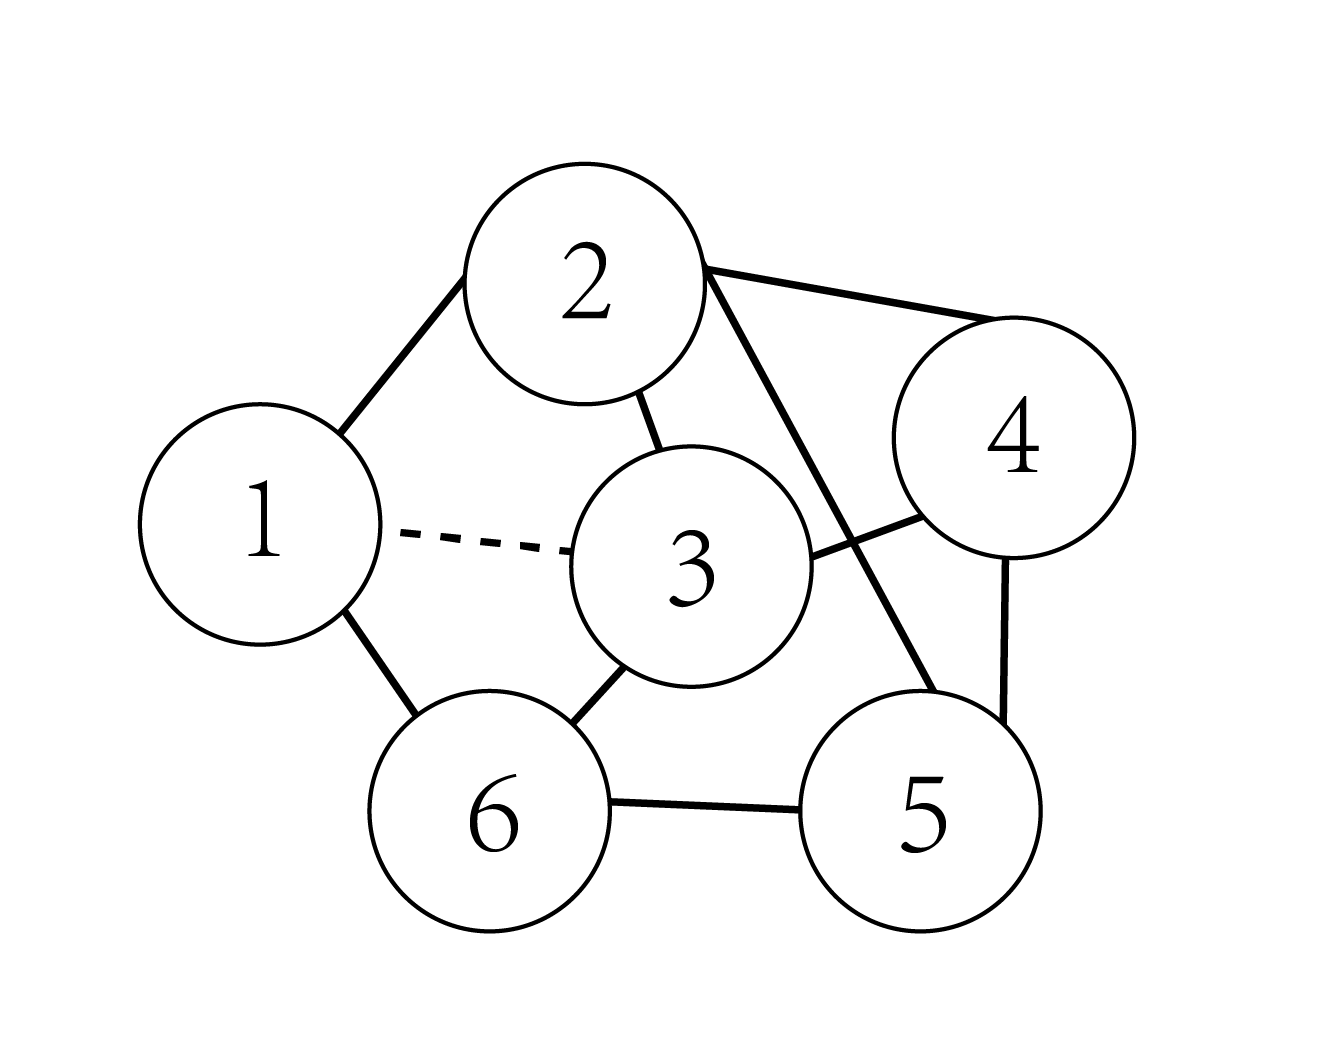
\includegraphics[width=3in]{figures/CN_incremental.png}}
	\caption{共同邻居矩阵变化的案例}
	\label{fig:case_for_lemma}
	\end{center}
\end{figure}
如图\ref{fig:case_for_lemma}中所示,图中虚线所示节点1和节点3之间的连边为新增的连边,根据图示可以得到邻接矩阵$\textbf{A}$为:
\begin{equation}
\begin{matrix}
	\textbf{A} = \begin{bmatrix}
	0&1&0&0&0&1 \\
	1&0&1&1&1&0\\
	0&1&0&1&0&1 \\
	0&1&1&0&1&0\\
	0&1&0&1&0&1\\
	1&0&1&0&1&0
	\end{bmatrix} ,
	\Delta\textbf{A} = \begin{bmatrix}
	0&0&\textbf{1}&0&0&0 \\
	0&0&0&0&0&0\\
	\textbf{1}&0&0&0&0&0 \\
	0&0&0&0&0&0\\
	0&0&0&0&0&0\\
	0&0&0&0&0&0
	\end{bmatrix}
\end{matrix}
\end{equation}
根据$\textbf{S}_{CN} = \textbf{A}\textbf{A}-\textbf{D}$,通过计算不同时刻的矩阵$\textbf{S}_{CN}$,可以计算得到$\Delta \textbf{S}_{CN}$的具体矩阵:
\begin{equation}
\Delta \textbf{S}_{CN} = \textbf{S}_{CN}^{(t+1)}- \textbf{S}_{CN} = \begin{bmatrix}
0&\textbf{1}&0&\textbf{1}&0&\textbf{1} \\
\textbf{1}&0&\textbf{1}&0&0&0\\
0&\textbf{1}&0&0&0&\textbf{1} \\
\textbf{1}&0&0&0&0&0\\
0&0&0&0&0&0\\
\textbf{1}&0&\textbf{1}&0&0&0
\end{bmatrix}
\end{equation}
其中节点1和节点3的邻居集合分别为$N(1) = {2,6}$,$N(3) = {2,4,6}$,则对应地,在$\Delta \textbf{S}_{CN}$中$(1,2),(1,4),(1,6),(3,2),(3,6)$及对应的对称元素为1。

\begin{lemma}
	{对角矩阵$\textbf{D}'$的变化}:在网络中节点总数不变时,网络中增加或删除一条边$(i,j)$,假设节点$i,j$的邻居集合分别为$N(i), N(j)$,且有$|N(i) \cup N(j)|=n$, 则对角矩阵$\textbf{D}'$中变化的元素个数为$n+2$,也即$\Delta\textbf{D}'$中非零元素个数为$n+2$,不同位置$k$对应值不同,对于非零元素的具体情况如下:
	\begin{equation}
		\Delta\textbf{D}'_{kk}=\left\{
		\begin{array}{ccl}
		1       &      & k\in N(i)\setminus N(j)\quad or\quad  k\in N(j)\setminus N(i)\\
		2     &      & k\in N(j) \cap N(i)\\
		|N(i)|     &      & k=j\\
		|N(j)|       &      & k=i 
		\end{array} \right.
	\end{equation}
\end{lemma}
根据\textbf{算法3.1}中$\textbf{D}'$的定义,得出矩阵$\textbf{D}'$的变化量可以根据$\textbf{S}$推算而来,上述引理的证明就不再赘述。

上述两个引理中,分别通过常数复杂度计算出$\Delta\textbf{S}_{CN}$和$\Delta\textbf{D}'$,根据式(\ref{defin:delta_w}),对时刻$t+1$有:
\begin{equation}
	\begin{aligned}
	\textbf{W} + \Delta\textbf{W} &= (\textbf{D}'+\Delta\textbf{D}')^{-\frac{1}{2}}(\textbf{S}_{CN}+\Delta\textbf{S}_{CN})(\textbf{D}'+\Delta\textbf{D}')^{-\frac{1}{2}} \\	
	\end{aligned}
\end{equation}
注意到其中矩阵$\textbf{D}'$为对角矩阵,从$\textbf{D}'$和$\Delta\textbf{D}'$容易推导出$\Delta\textbf{D}^{\prime-\frac{1}{2}}$,因此将上式改写为:
\begin{equation}
	\begin{aligned}
	\textbf{W} + \Delta\textbf{W} &= (\textbf{D}^{\prime-\frac{1}{2}}+\Delta\textbf{D}^{\prime-\frac{1}{2}})(\textbf{S}_{CN}+\Delta\textbf{S}_{CN})(\textbf{D}^{\prime-\frac{1}{2}}+\Delta\textbf{D}^{\prime-\frac{1}{2}}) \\	
	& = \textbf{D}^{\prime-\frac{1}{2}}\textbf{S}_{CN}\textbf{D}^{\prime-\frac{1}{2}}+
	\textbf{D}^{\prime-\frac{1}{2}}\textbf{S}_{CN}\Delta\textbf{D}^{\prime-\frac{1}{2}}+
	\textbf{D}^{\prime-\frac{1}{2}}\Delta\textbf{S}_{CN}\textbf{D}^{\prime-\frac{1}{2}}+
	\Delta\textbf{D}^{\prime-\frac{1}{2}}\textbf{S}_{CN}\textbf{D}^{\prime-\frac{1}{2}}\\
	&+\textbf{D}^{\prime-\frac{1}{2}}\Delta\textbf{S}_{CN}\Delta\textbf{D}^{\prime-\frac{1}{2}}+
	\Delta\textbf{D}^{\prime-\frac{1}{2}}\Delta\textbf{S}_{CN}\textbf{D}^{\prime-\frac{1}{2}}+
	\Delta\textbf{D}^{\prime-\frac{1}{2}}\textbf{S}_{CN}\Delta\textbf{D}^{\prime-\frac{1}{2}}+\\
	&+\Delta\textbf{D}^{\prime-\frac{1}{2}}\Delta\textbf{S}_{CN}\Delta\textbf{D}^{\prime-\frac{1}{2}}
	\end{aligned}
\end{equation}
根据矩阵计算理论\cite{golub2012matrix},去掉上式中对实际结果影响较小的高阶增量项,同时考虑到式(\ref{defin:delta_w})中矩阵$\textbf{W}= \textbf{D}^{\prime-\frac{1}{2}}\textbf{S}_{CN}\textbf{D}^{\prime-\frac{1}{2}}$,则对于$\Delta\textbf{W}$有:
\begin{equation}
	\Delta\textbf{W}= \textbf{D}^{\prime-\frac{1}{2}}\textbf{S}_{CN}\Delta\textbf{D}^{\prime-\frac{1}{2}}+
	\textbf{D}^{\prime-\frac{1}{2}}\Delta\textbf{S}_{CN}\textbf{D}^{\prime-\frac{1}{2}}+
	\Delta\textbf{D}^{\prime-\frac{1}{2}}\textbf{S}_{CN}\textbf{D}^{\prime-\frac{1}{2}}
\end{equation}
在上式中一阶增量$\Delta\textbf{S}_{CN}$和$\Delta\textbf{D}^{\prime-\frac{1}{2}}$中只有个别元素非零,且因$\Delta\textbf{D}^{\prime-\frac{1}{2}}$为对角矩阵,因此可以通过上式充分简化$\Delta\textbf{W}$的计算。

下面将对网络增量的第二种情况进行分析:节点新增
%%%%%%%%%%%%%%%%%%%%%%%%%%%%%%%%%%%%%%%
%----------------------------------------     节点新增    ---------------------------------------%
%%%%%%%%%%%%%%%%%%%%%%%%%%%%%%%%%%%%%%%
\subsection{节点新增}
网络中节点的新增往往伴随着网络中连边的增加,因此这一个过程可以视为两个过程的叠加:
\begin{itemize}
	\item 节点新增
	\item 节点数不变,新增连边
\end{itemize}
第二个过程在前文中已经做了详细的分析和算法设计,第一个过程中节点新增需要对原有表征向量矩阵进行增广,由于跟新增任何节点没有连接,于是需要补0进行增广。针对有节点新增情况的网络增量学习算法iHLE-na过程具体见\textbf{算法3.3}。通过对比算法流程上的差异,根据是否有新增节点,算法流程上只需对原表征向量进行增广即可,因此iHLE-nn算法和iHLE-na算法之间是可以互相推论的,故在后文统一称为算法iHLE。


\begin{figure}[htb]
	\centering
	\begin{minipage}{.7\linewidth}
		\begin{algorithm}[H]\label{iHLE_na}
			\small
			\caption{iHLE-na算法}
			\begin{algorithmic}[1]
				\Require
				\Statex $\textbf{X} ^{(t)},\Lambda^{(t)}$ :网络在时刻$t$的网络表征结果和特征值对角矩阵
				\Statex $\Delta\textbf{W}$ :网络从时刻$t$到$t+1$的矩阵$\textbf{W}$的变化量
				\Statex $k$ : 表征向量维数
				\Ensure
				\Statex $\textbf{X}^{(t+1)T}$ :时刻$t+1$的网络表征向量矩阵
				\Statex $\Lambda^{(t+1)}$:时刻$t+1$网络对应的特征值对角矩阵
				\Statex
				\State 对$\Delta\textbf{W}$特征值分解,$\Delta\textbf{W} =  \textbf{Y}^{T} \textbf{Z}  \textbf{Y}$
				\State 对$ \textbf{X}^{(t)T}$进行补0增广,增加一行0。
				\State 对$\begin{bmatrix} \textbf{X}^{(t)T} & \textbf{Y}^{T}\end{bmatrix}$进行QR分解,$\begin{bmatrix} \textbf{X}^{(t)T} & \textbf{Y}^{T}\end{bmatrix} = \begin{bmatrix} \textbf{X}^{(t)T} & \Delta\textbf{Q}^{T} \end{bmatrix} \textbf{R}$
				\State 令$\textbf{M} = \textbf{R}\begin{bmatrix}  \Lambda^{(t)} & \textbf{0};
				\textbf{0} & \textbf{Z} \end{bmatrix}
				\textbf{R}^T$
				\State 对$\textbf{M}$进行特征值分解,取前k个特征值对应的特征向量;$\textbf{M} =\textbf{V}^T \Lambda^{(t+1)} \textbf{V}$
				\State $\textbf{X}^{(t+1)T} = \begin{bmatrix} \textbf{X}^{(t)T} & \Delta\textbf{Q}^{T} \end{bmatrix} \textbf{V}^T$
				\State 返回 $\textbf{X}^{(t+1)T}, \Lambda^{(t+1)}$
			\end{algorithmic}
		\end{algorithm}
	\end{minipage}
\end{figure}

%%%%%%%%%%%%%%%%%%%%%%%%%%%%%%%%%%%%%%%
%----------------------------------------     本章小结     ---------------------------------------%
%%%%%%%%%%%%%%%%%%%%%%%%%%%%%%%%%%%%%%%
\section{本章小结}
本章首先基于拉普拉斯特征映射方法只能保留一阶接近度的问题,提出了基于高阶接近度的图表征算法HLE。考虑到网络的动态变化过程,本章对网络动态变化过程分成两种情况进行讨论:节点不变和节点增量情况;通过对算法输入的网络中增量矩阵的分析和计算,提出增量情况下的网络表征算法iHLE,并提供了一种从邻接矩阵优化算法输入的增量矩阵的思路。

